\chapter{Opis użytych algorytmów}

\section{Odległość Levensteina}

\begin{figure} [H]
	\centering
	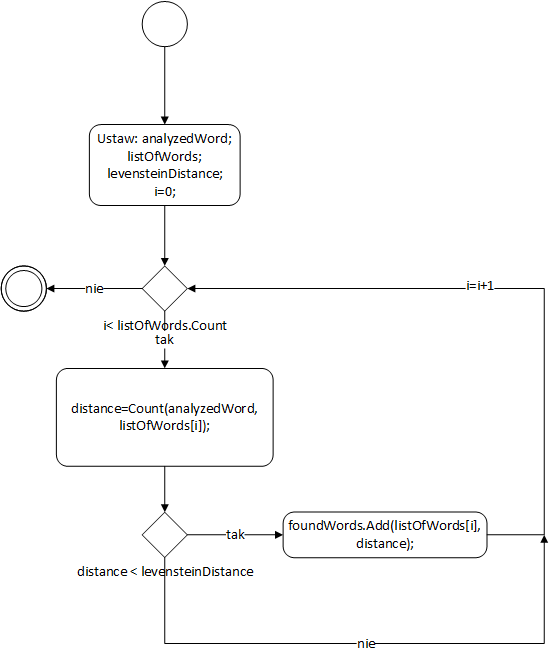
\includegraphics[width=0.6\linewidth]{rozdzial02/Levenstein1.png}
	\caption{Diagram dla działania algorytmu z wykorzystaniem odległości Levensteina}
	\label{fig:Lev}
\end{figure}

\begin{figure} [H]
	\centering
	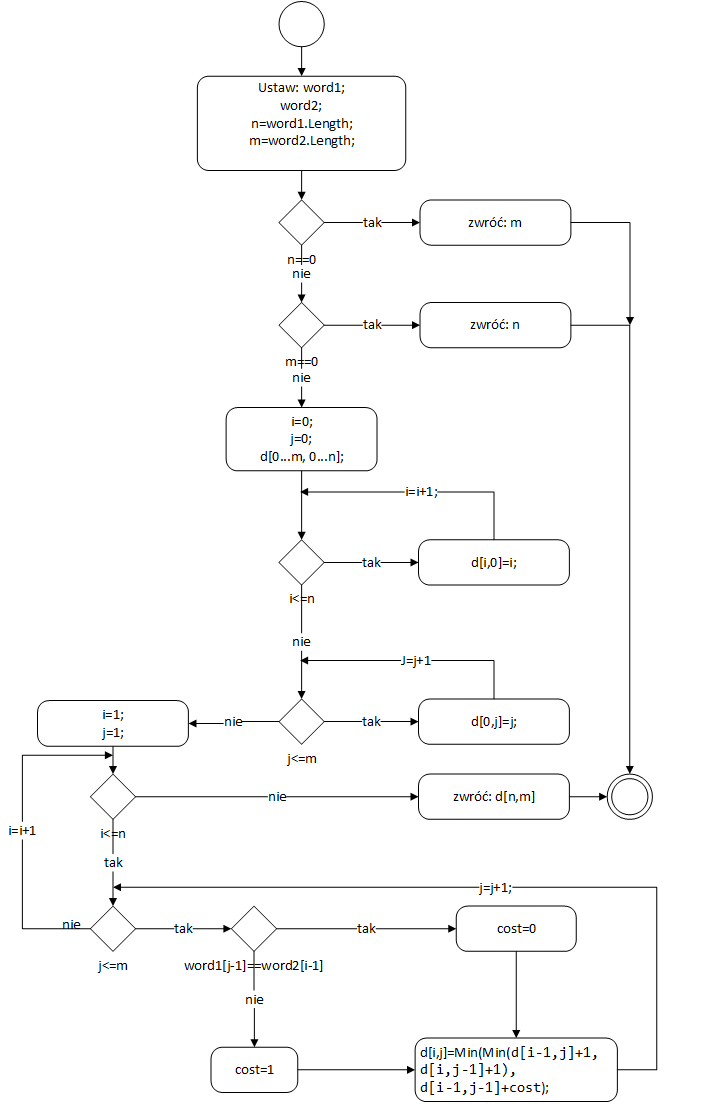
\includegraphics[width=1\linewidth]{rozdzial02/Levenstein-Count.png}
	\caption{Diagram obliczania odległości Levensteina}
	\label{fig:Lev-Count}
\end{figure}


\section{LetterChanger}

\section{SpaceAdder}

\begin{figure} [H]
	\centering
	
\includegraphics[width=0.6\linewidth]{rozdzial02/SpaceSearcher.png}
	\caption{Diagram działania funkcji dodającej przerwy między wyrazami}
	\label{fig:SpaceAdder}
\end{figure}



